\section{Experiments}


We validate our approach in this section with extensive empirical analysis using three popularly used domain generalization benchmarks. We follow this up with a detailed analysis of the behavior of ALT and its constituent parts. 


\paragraph{Datasets.}
The SSDG setup is as follows: we train on a single dataset as the source domain, and evaluate its performance on unobserved target (or test) domains with no access to any data from them during training. We demonstrate the effectiveness of our approach using three popular domain generalization benchmark datasets which we describe next -- (a) \textit{Digits}, we use follow the setting from Volpi~ \textit{et al.}~\citep{volpi2018generalizing} and use 1000 images from MNIST~\citep{lecun1998mnist} as the source dataset, and USPS~\citep{denker1988neural}, SVHN~\citep{netzer2011reading}, MNIST-M and SYNTH~\citep{ganin2015unsupervised} as the target datasets; (b) \textit{PACS:} Our second benchmark is the PACS dataset~\citep{li2017deeper} which consists of images belonging to 7 classes from 4 domains (P: photo, A: art painting, C: cartoon, S: sketch); and finally (c) \textit{Office-Home:} Our third benchmark is OfficeHome~\citep{venkateswara2017deep}, which consists of images belonging to 65 classes from 4 domains (A: art, C: clipart, R: real, P: product). 
%In all of these cases, we train models on each individual domain, while testing on the remaining domains and report the average accuracy across all domains as the domain generalization performance of the benchmark, repeated over for 5 random seeds.

\paragraph{Evaluation.}
For all datasets, we train models on each individual domain, while testing on the remaining domains. We provide fine-grained results on each test set as well as the average domain generalization performance. Accuracy is reported as the mean over 5 repetitions of the experiment with random seeds. We compare with several state-of-the-art techniques on single source domain generalization and compare three variants of our methods: ALT$_{g-only}$ refers to the simplest form of our method that only uses the adversary network during training without an explicit diversity module $r$. ALT$_{RandConv}$ and ALT$_{AugMix}$ utilize RandConv and AugMix, respectively, as the diversity module, where the consistency is now placed 
% on three terms 
as explained in \eqref{alt:eq:L_KL}.
% We report the mean and standard deviation of performance for 5 repetitions,


\begin{table}[t]
    \centering
    % \small
    \resizebox{\linewidth}{!}{
    \begin{tabular}{@{}l lllll l @{}}
        \toprule
        \textbf{Method} & \textbf{MNIST-10K} & \textbf{MNIST-M} & \textbf{SVHN} & \textbf{USPS} & \textbf{SYNTH} & \textbf{Target Avg.} \\ % & \textbf{Digits Avg.} \\
        \midrule
        ERM                                 & 98.40 {\footnotesize$\pm$ 0.84} & 58.87 {\footnotesize$\pm$ 3.73 } & 33.41 {\footnotesize$\pm$ 5.28 } & 79.27 {\footnotesize$\pm$ 2.70 } & 42.43 {\footnotesize$\pm$ 5.46 } & 53.50 {\footnotesize$\pm$ 4.23 } \\
        % & 62.48 {\footnotesize$\pm$ }\\
        ADA~\citep{volpi2018generalizing}    &  N/A  & 60.41 & 35.51 & 77.26 & 45.32 & 54.62 \\ % & \\
        M-ADA~\citep{qiao2020learning}       & 99.30 & 67.94 & 42.55 & 78.53 & 48.95 & 59.49 \\ % & \\
        AugMix~\citep{hendrycks2019augmix}   & 98.53 {\footnotesize$\pm$ 0.18} & 53.36 {\footnotesize$\pm$ 1.59} & 25.96 {\footnotesize$\pm$ 0.80} & 96.12 {\footnotesize$\pm$ 0.72} & 42.90 {\footnotesize$\pm$ 0.60} & 54.59 {\footnotesize$\pm$ 0.50}\\
        RandConv~\citep{xu2020robust}        & 98.85 {\footnotesize$\pm$ 0.04 } & 87.76 {\footnotesize$\pm$ 0.83} &	57.62 {\footnotesize$\pm$ 2.09} & 83.36 {\footnotesize$\pm$	0.96} & 62.88 {\footnotesize$\pm$ 0.78} & 72.88 {\footnotesize$\pm$ 0.58} \\
        \midrule 
        ALT$_{g-only}$                      & 98.46 {\footnotesize$\pm$0.27} & 74.28 {\footnotesize$\pm$1.36} & 52.25 {\footnotesize$\pm$1.54} & 94.99 {\footnotesize$\pm$0.68} & 68.44 {\footnotesize$\pm$0.98} & 72.49{\footnotesize$\pm$ 0.87} \\
        ALT$_{RandConv}$                    & 98.46 {\footnotesize$\pm$ 0.25} & 76.90 {\footnotesize$\pm$ 1.42} & 53.78 {\footnotesize$\pm$ 1.97} & 95.40 {\footnotesize$\pm$ 0.72} & 69.40 {\footnotesize$\pm$ 1.07} & \textbf{73.87} {\footnotesize$\pm$ 1.03}\\
        ALT$_{AugMix}$                      & 98.55 {\footnotesize$\pm$ 0.11} & 75.98 {\footnotesize$\pm$ 0.59} & 55.01 {\footnotesize$\pm$ 1.34} & 96.17 {\footnotesize$\pm$ 0.45} & 69.93 {\footnotesize$\pm$ 2.17} & \textbf{74.38} {\footnotesize$\pm$ 0.86}\\
        \bottomrule
    \end{tabular}
    }
    \caption{Single-source domain generalization accuracy (\%) on digit classification, with MNIST-10K as source and MNIST-M, SVHN, USPS, and SYNTH as target domains. Performance reported over five repetitions. Note:ADA and M-ADA do not report standard deviation.}
    \label{tab:results_digits}
\end{table}
\subsection{Digits}
\paragraph{Baselines.}
Our baselines include a na\"ive ``source-only'' baseline which is trained using expected risk minimization (ERM) on the source dataset, M-ADA~\citep{qiao2020learning} -- an adversarial data augmentation method, and AugMix~\citep{hendrycks2019augmix} 
and RandConv~\citep{xu2020robust} which exploit diversity through consistency constraints.
We use DigitNet~\citep{volpi2018generalizing} as the model architecture for all models for a fair comparison.
All models are trained for $T{=}10000$ iterations, with batch-size of $32$, learning rate of $0.0001$, using the \texttt{Adam} optimizer.
For ALT, we set the consistency coefficient $\lambda_{KL}{=}0.75$, adversarial learning rate $\eta_{adv}{=}5e{-}6$, number of adversarial steps $m_{adv}{=}10$, and equal weight $w_r{=}1.0$ for diversity and adversary networks.

\paragraph{Results.}
Table~\ref{tab:results_digits} shows the comparison between our method and prior art on the Digits benchmark.
Previous pixel-level adversarial training approaches (ADA and M-ADA) offer only marginal improvements over the na\"ive ERM baseline. The results for diversity-promoting data augmentation methods are mixed -- while AugMix is only $1.09\%$ better than ERM, RandConv provides a significant boost. Interestingly, the base version of our approach, ALT$_{g-only}$, which is exclusively based on adversarial training, is significantly better than pixel-level adversarial training.
More importantly, it is also better than diversity method AugMix, while performing lower than RandConv by a small margin $-0.39\%$.
When we trained ALT with  adaptive diversity (ALT$_{RandConv}$ and ALT$_{AugMix}$), we achieved the best performance, beating previous state-of-the-art by $0.99\%$ and $1.50\%$ respectively.
The hardest target domains on this benchmark have been SVHN and SYNTH, both of which are obtained from real-world images of street signs or house number signs.
On the other hand, USPS is closely correlated with MNIST, both being black-and-white, centered images of handwritten digits, while MNIST-M is derived from MNIST but with different backgrounds. AugMix fares poorly on both real-world datasets, but is able to generalize well to MNIST-M and USPS. However ALT is able to use its adversary network in combination with AugMix, resulting in an overall improvement.

\begin{figure*}
    \centering
    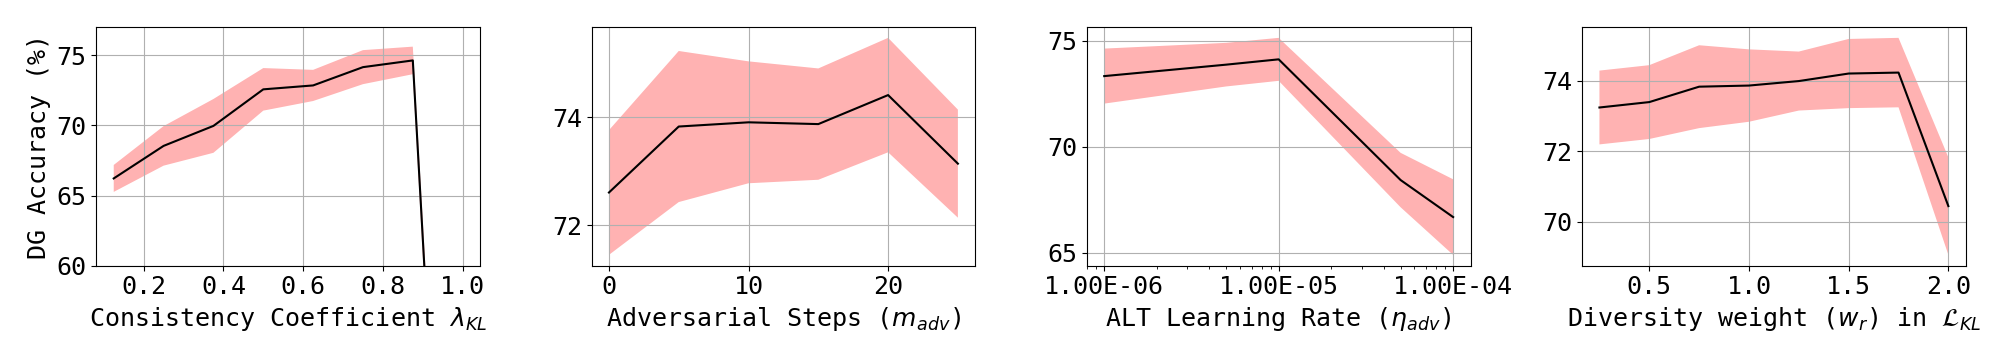
\includegraphics[width=\linewidth]{alt/figures/digits_hyperparam.png}
    \caption{\small{\textbf{Ablation Analysis:} We study the effect of each hyper-parameter in ALT on the average accuracy using the Digits benchmark. For each experiment we show 1 standard deviation around the mean over 5 runs. We observe that the consistency (left most) is generally important until a certain point, after which it becomes harmful; (left center) taking more adversarial steps improves performance; (right center) similarly, a small learning rate is preferred in training the adversary network, $g$, and performance degrades as the learning rate increases; (right most) Surprisingly, we find that the trade-off between diversity and ALT is non- trivial and dataset dependent.}}
    \label{fig:digits_hp}
\end{figure*}

\begin{table*}[t]
    \centering
    % \small
    \resizebox{\linewidth}{!}{
    \begin{tabular}{@{}l ccc ccc ccc ccc c@{}}
        \toprule
        \textbf{Method} & \textbf{A$\rightarrow$C} & \textbf{A$\rightarrow$S} & \textbf{A$\rightarrow$P} & \textbf{C$\rightarrow$A} & \textbf{C$\rightarrow$S} & \textbf{C$\rightarrow$P} & \textbf{S$\rightarrow$A} & \textbf{S$\rightarrow$C} & \textbf{S$\rightarrow$P} & \textbf{P$\rightarrow$A} & \textbf{P$\rightarrow$C} & \textbf{P$\rightarrow$S} & \textbf{Average}\\
        \midrule
        ERM                                 & 62.3 & 49.0 & 95.2 & 65.7 & 60.7 & 83.6 & 28.0 & 54.5 & 35.6 & 64.1 & 23.6 & 29.1 & 54.3\\
        JiGen~\citep{carlucci2019domain}     & 57.0 & 50.0 & 96.1 & 65.3 & 65.9 & 85.5 & 26.6 & 41.1 & 42.8 & 62.4 & 27.2 & 35.5 & 54.6\\
        ADA~\citep{volpi2018generalizing}    & 64.3 & 58.5 & 94.5 & 66.7 & 65.6 & 83.6 & 37.0 & 58.6 & 41.6 & 65.3 & 32.7 & 35.9 & 58.7 \\
        AugMix~\citep{hendrycks2019augmix}   & 68.4 & 54.6 & 95.2 & 74.3 & 66.7 & 87.3 & 40.0 & 57.4 & 46.8 & 67.3 & 26.8 & 41.4 & 59.6 \\
 
        RandConv~\citep{xu2020robust}        & 61.1 & 60.5 & 87.3 & 57.1 & 72.9 & 73.7 & 52.2 & 63.9 & 46.1 & 61.3 & 37.6 & 50.5 & 60.3\\
        SagNet~\citep{nam2021reducing}       & 67.1 & 56.8 & 95.7 & 72.1 & 69.2 & 85.7 & 41.1 & 62.9 & 46.2 & 69.8 & 35.1 & 40.7 & 61.9 \\
        \midrule 
        ALT$_{g-only}$                  & 63.5 & 63.8 &	94.9 & 68.9 & 74.4 & 84.6 & 39.7 & 61.1 & 49.3 &	68.8 & 43.4 & 50.8 & \textbf{63.6}\\
        ALT$_{RandConv}$                    & 63.6 & 65.8 & 92.5 & 69.1 & 75.1 & 84.5 & 40.1 & 61.7 & 50.8 & 68.4 & 43.4 & 55.2 & \textbf{64.2}\\
        ALT$_{AugMix}$                      & 65.7 & 68.2 & 93.2 & 71.9 & 74.2 & 86.0 & 40.2 & 62.9 & 49.1 & 68.5 & 43.5 & 53.3 & \textbf{64.7}\\
        % AugMax                            & 85.4 & 79.6 & 90.1 & 77.1 & 77.4 & 84.3 & 37.0 & 41.9 & 45.9 & 66.8 & 54.6 & 53.5 & 66.1 \\
        \bottomrule 
    \end{tabular}
    }
    \caption[SSDG PACS]{
        Single-source domain generalization accuracy (\%) on PACS~\citep{csurka2017domain}. 
        \textit{X$\rightarrow$Y} implies X is the source dataset and Y is the target dataset.
        \textit{P: photo; A: art-painting; C: cartoon; S: sketch.}
        Performance is reported as mean of 5 repetitions\footnotemark[1].
    }
    \label{tab:results_pacs}
\end{table*}


\subsection{PACS}
\footnotetext{$^*$standard deviation values are in the supplementary material.}
\paragraph{Baselines.}
Our baselines include JiGen~\citep{carlucci2019domain}, adversarial data augmentation (ADA)~\citep{volpi2018generalizing}, AugMix, RandConv, and SagNet~\citep{nam2021reducing} which is designed to reduce style bias using normalization techniques.
We use ResNet18~\citep{he2016deep} pre-trained on ImageNet as our model architecture and train all models for $2000$ iterations with batch-size of $32$, learning rate $0.004$, \texttt{SGD} optimizer with cosine annealing learning rate scheduler, weight decay of $0.0001$, and momentum $0.9$.
For ALT, we set consistency coefficient $\lambda_{KL}{=}0.75$, adversarial learning rate $\eta_{adv}{=}5e{-}5$, number of adversarial steps $m_{adv}{=}10$ and $w_r{=}1.0$.

\paragraph{Results.}
Results are shown in Table~\ref{tab:results_pacs}.
We observe that ALT without a diversity module (ALT$_{g-only}$) surpasses generalization performance of all prior methods including diversity methods RandConv and AugMix and the previous best SagNet~\citep{nam2021reducing}.
ALT with adaptive diversity further improves the results and ALT$_{AugMix}$ establishes a new state-of-the-art accuracy of $64.7\%$.
The most difficult target domains for previous methods has been \textit{Sketch (S)} since this is a set of rough human-drawn black-and-white sketches of real-life objects; the difficluty can be observed in terms of performance in columns $A{\rightarrow}S$, $C{\rightarrow}S$, and $P{\rightarrow}S$.
ALT significantly improves the performance on the sketch target domain, compared to the previous best.
ALT is also the best when generalizing from photos as the source to C,S,A as targets.
This is a very realistic setting since large-scale natural image datasets such as ImageNet~\citep{deng2009imagenet} are widely used and publicly available, while datasets for sketches, cartoons, and painting are not.

\begin{table*}[t]
    \centering
    % \small
    \resizebox{\linewidth}{!}{
    \begin{tabular}{@{}l ccc ccc ccc ccc c@{}}
        \toprule
        \textbf{Method} & \textbf{A$\rightarrow$C} & \textbf{A$\rightarrow$P} & \textbf{A$\rightarrow$R} & \textbf{C$\rightarrow$A} & \textbf{C$\rightarrow$P} & \textbf{C$\rightarrow$R} & \textbf{P$\rightarrow$A} & \textbf{P$\rightarrow$C} & \textbf{P$\rightarrow$R} & \textbf{R$\rightarrow$A} & \textbf{R$\rightarrow$C} & \textbf{R$\rightarrow$P} & \textbf{Average}\\
        \midrule
        ERM                                 & 42.61 & 59.18 & 69.45 & 48.37 & 56.09 & 59.38 & 46.07 & 40.18 & 68.19 & 63.12 & 45.13 & 74.34 & 56.00 \\
        AugMix~\citep{hendrycks2019augmix}   & 45.31 & 61.88 & 71.88 & 49.30 & 58.93 & 62.24 & 50.04 & 42.59 & 71.51 & 64.10 & 47.56 & 75.95 & 58.44 \\
        RandConv~\citep{xu2020robust}    & 43.98 & 55.28 & 67.31 & 45.49 & 56.58 & 59.03 & 43.80 & 43.19 & 66.50 & 57.62 & 48.26 & 72.97 & 55.00\\
        SagNet~\citep{nam2021reducing}   & 42.18 & 56.03 & 67.34 & 46.68 & 53.89 & 57.88 & 45.49 & 40.09 & 67.11 & 61.39 & 48.32 & 72.79 & 54.93\\
        \midrule 
        ALT$_{g-only}$                  & 47.26 & 61.14 & 71.21 & 48.88	& 57.81 & 60.99	& 48.15 & 46.70 & 69.30 & 64.85 & 52.84 & 76.28 & \textbf{58.78} \\
        ALT$_{RandConv}$                & 48.33 & 61.19 & 71.75 & 50.13 & 58.82 & 62.26 & 49.21 & 47.03 & 70.53 & 64.88 & 53.10 & 76.07 & \textbf{59.44}\\
        ALT$_{AugMix}$                  & 48.06 & 61.16 & 71.12 & 50.43 & 58.84 & 61.84 & 49.32 & 47.55 & 70.64 & 64.86 & 53.27 & 76.29 & \textbf{59.45} \\
        \bottomrule 
    \end{tabular}
    }
    \caption[SSDG Office-Home]{Single-source domain generalization accuracy (\%) on Office-Home~\citep{venkateswara2017deep} 
    % with mean and standard deviation 
    over five repetitions. 
    \textit{X$\rightarrow$Y} implies X is the source dataset and Y is the target dataset.
    \textit{R: real; A: art; C: clipart; P: product.}
    Performance is reported as mean of 5 repetitions\footnotemark[1].
    % ; detailed results with standard deviation values are in the supplementary material.
    }
    \label{tab:results_officehome}
\end{table*}
\subsection{Office-Home}
\paragraph{Baselines.}
For PACS, we follow the protocol from the previous state-of-the-art Sagnet~\citep{nam2021reducing} and use ResNet50 as the model architecture.
% and identical training settings and hyperparameters as PACS.
Note that we do not perform any hyperparameter tuning for OfficeHome and directly apply identical training settings and hyperparameters from PACS.

\paragraph{Results.}
Table~\ref{tab:results_officehome} shows the results on Office-Home.
We observe that RandConv (previous best on Digits) and SagNet (previous best on PACS) perform worse than ERM on OfficeHome, while AugMix is better by $2.44\%$.
All three variants of ALT surpass prior results, with ALT$_{AugMix}$ resulting in the best accuracy of $59.45\%$.
The most difficult target domain for previous methods are \textit{Art (A)} and \textit{Clipart (C)}, possibly because both sets have images with white backgrounds, while real world photos (R) and product images are naturally occurring.
ALT improves performance in each case when with A or C as target domain.
An observation similar to PACS can also be made here -- ALT is the best model under the realistic setting of generalizing from widely available real photos (R) to other domains.
